%!TEX encoding = UTF-8 Unicode
%!TEX root = ../lect-week06.tex

%%%

\Subsection{Vad är en klass?}

\begin{Slide}{Vad är en klass?}
\begin{itemize} 
\item En klass är en mall för att skapa objekt. 
\item Objekt skapas med \code{new Klassnamn} och kallas för  \Emph{instanser} av klassen \code{Klassnamn}.
\item En klass innehåller medlemmar \Eng{members}: 
  \begin{itemize} 
  \item \Emph{attribut}, kallas även fält \Eng{field}: \code{val}, \code{lazy val}, \code{var} 
  \item \Emph{metoder}, kallas även operationer: \code{def}
  \end{itemize}
\item Varje instans har sin uppsättning värden på attributen (fälten).
\end{itemize}

\end{Slide}


\ifkompendium\else


\begin{Slide}{Vad är en klass?}\SlideFontSmall
Metafor: En klass liknar en \Emph{stämpel}
\begin{figure}
\centering
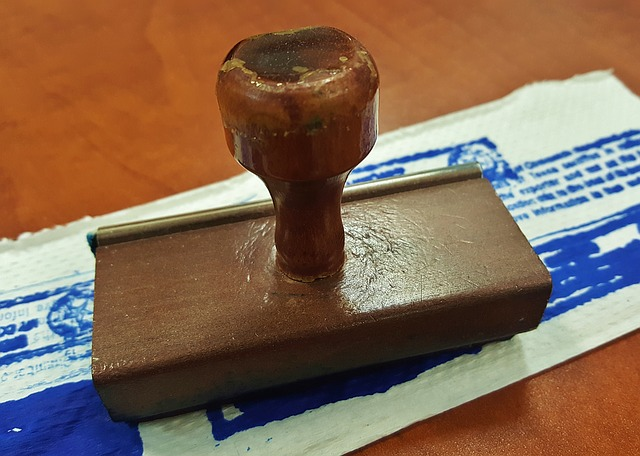
\includegraphics[width=0.5\textwidth]{../img/stamp}
\end{figure}
\begin{itemize}
\item En stämpel kan tillverkas -- motsvarar deklaration av klassen. 
 \item Det händer inget förrän man stämplar -- motsvarar \code{new}.
\item Då skapas avbildningar -- motsvarar instanser av klassen.


\end{itemize}
\end{Slide}


\begin{Slide}{Klassdeklarationer och instansiering}\SlideFontSmall
\setlength{\leftmargini}{0pt}
\begin{itemize}
\item Syntax för deklaration av klass: \\ \vspace{0.5em}{\SlideFontSize{13}{16}\code|class Klassnamn(parametrar){ medlemmar }|}\vspace{0.5em}



\item Exempel \Emph{deklaration}:
\begin{Code}
class Klassnamn(val attribut1: Int, attribut2: String){  
  val attribut3: Double = 42.0              //publikt oföränderligt attribut
  private var attribut3: Boolean = false    //privat medlem syns inte utåt
  def metod(parameter: Int) = parameter + 1 //funktion i klass kallas metod
  lazy val attr4 = Vector.fill(100000)(42.0)     //fördröjd initialisering 
}
\end{Code}

\item Parametrar initialiseras med de argument som ges vid \code{new}. 
\item Exempel \Emph{instansiering}:
\begin{Code}
val instansReferens = new Klassnamn(42, "hej")
\end{Code}

\item Attribut blir \Emph{publika} (alltså synliga utåt) om inte modifieraren \code{private} anges.
\item Parametrar som inte föregås av modifierare (t.ex. private val, val, var) blir attribut som är: \code{ private[this] val } och bara synliga i \Alert{denna} instans.

\end{itemize}
\end{Slide}


\begin{Slide}{Exempel: Klassen Complex i Scala}\SlideFontSmall
\begin{Code}
class Complex(val re: Double, val im: Double){
  def r  = math.hypot(re, im)
  def fi = math.atan2(re, im)
  def +(other: Complex) = new Complex(re + other.re, im + other.im)
  var imSymbol = 'i'
  override def toString = s"$re + $im$imSymbol"
}
\end{Code}

\begin{REPL}
scala> val c1 = new Complex(3, 4)
c1: Complex = 3.0 + 4.0i

scala> val polarForm = (c1.r, c1.fi)
polarForm: (Double, Double) = (5.0,0.6435011087932844)

scala> val c2 = new Complex(1, 2)
c2: Complex = 1.0 + 2.0i

scala> c1 + c2
res0: Complex = 4.0 + 6.0i
\end{REPL}

%TODO:
%  \begin{itemize} 
%  \item Bygg upp \code{case class Complex(re: Double, im: Double)} steg för steg inspirerat av Pins3ed kap 6 i likhet med hur de gör med Rational
%  \item Illustrera följande begrepp: this (behövs i max(that)), method overloading behövs för att plussa med både Complex och Double
%  \item Till fördjupningsövning: dekorera Double med metoderna im och re samt (Double, Double) med metoden ir (för irrational) med implicit klass
%  \item Till extrauppgift: implementera klassen Polar(r, fi) med polära koordinater \url{https://sv.wikipedia.org/wiki/Pol%C3%A4ra_koordinater}
%  \end{itemize}
\end{Slide}

\begin{Slide}{Exempel: Principen om enhetlig access}\SlideFontSmall
\begin{Code}
class Complex(val re: Double, val im: Double){
  val r  = math.hypot(re, im)
  val fi = math.atan2(re, im)
  def +(other: Complex) = new Complex(re + other.re, im + other.im)
  var imSymbol = 'i'
  override def toString = s"$re + $im$imSymbol"
}
\end{Code}
\pause
\begin{itemize}
\item Efter som attributen \code{re} och \code{im} är oföränderliga, kan vi lika gärna ändra i klass-implementationen och göra om metoderna \code{r} och \code{fi} till \code{val}-variabler utan att klientkoden påverkas. 

\item Då anropas \code{math.hypot} och \code{math.atan2} bara en gång vid initialisering (och inte varje gång som med \code{def}).

\item Vi skulle även kunna använda \code{lazy val} och då bara räkna ut \code{r} och \code{fi} om och när de verkligen refereras av klientkoden, annars inte.

\item Eftersom klientkoden inte ser skillnad på metoder och variabler, kallas detta \Emph{principen om enhetlig access}. (Många andra språk har \Alert{inte} denna möjlighet, tex Java.)

\end{itemize}

\end{Slide}


\begin{Slide}{Exempel: Motsvarande klass JComplex i Java}\SlideFontSmall
\javainputlisting[basicstyle=\SlideFontSize{5}{6}\ttfamily\selectfont]{../compendium/examples/JComplex.java}
\end{Slide}

\begin{Slide}{Exempel: Använda JComplex från Scala}
\begin{REPL}
$ javac JComplex.java 
$ scala
Welcome to Scala 2.11.8 (Java HotSpot(TM) 64-Bit Server VM, Java 1.8.0_66).
Type in expressions for evaluation. Or try :help.

scala> val jc1 = new JComplex(3, 4)
jc1: JComplex = 3.0 + 4.0i

scala> val polarForm = (jc1.getR, jc1.getFi)
polarForm: (Double, Double) = (5.0,0.6435011087932844)

scala> val jc2 = new JComplex(1, 2)
jc2: JComplex = 1.0 + 2.0i

scala> jc1 add jc2
res0: JComplex = 4.0 + 6.0i
\end{REPL}
\end{Slide}


\begin{Slide}{Exempel: Test av JComplex i Java}
\javainputlisting[basicstyle=\SlideFontSize{9}{11}\ttfamily\selectfont]{../compendium/examples/JComplexTest.java}
\begin{itemize}
\item Tupler finns inte i Java, så det går inte på ett enkelt sätt att i Java skapa par av värden somi Scala.

\item Operatornotation för metoder finns inte i Java, så man måste i Java använda punktnotation och skriva: \code{jc1.add(jc2)}
\end{itemize}
\end{Slide}


\Subsection{Instansiering: \texttt{new}}

\begin{Slide}{Instansiering med \texttt{new}}
Rita molbild med instanser av klassen Complex
\end{Slide}

\begin{Slide}{Instansiering med fabriksmetod}
\end{Slide}

\begin{Slide}{Instansiering med default-argument}
\end{Slide}

\begin{Slide}{Instansiering med alternativa fabriksmetoder}
\end{Slide}

\begin{Slide}{Förändringsbar eller oföränderlig?}
\end{Slide}


\Subsection{Referens saknas: \texttt{null}}

\begin{Slide}{Referens saknas: \texttt{null}}
\end{Slide}


\begin{Slide}{Konstruktor}
\end{Slide}

\begin{Slide}{Skräpsamling}
Destruktor
\end{Slide}

\Subsection{Synlighet}

\begin{Slide}{Synlighet}
definiera/förklara:
private
private[this]
\end{Slide}

\begin{Slide}{Kompanjonsobjekt}
\end{Slide}


\begin{Slide}{Synlighet av klassparametrar i klasser \& case-klasser}\SlideFontSmall
\code{private[this]} är \Alert{ännu} mer privat än \code{private} 
\begin{Code}
class Hemlis(private val hemlis: Int) {
  def ärSammaSom(annan: Hemlis) = hemlis == annan.hemlis   // Funkar!
}

class Hemligare(private[this] val hemlis: Int) {
  def ärSammaSom(annan: Hemligare) = hemlis == annan.hemlis //KOMPILERINGSFEL
}
\end{Code}
Vad händer om man inte skriver något? Olika för klass och case-klass:
\begin{Code}
class Hemligare(hemlis: Int) { // motsvarar private[this] val
  def ärSammaSom(annan: Hemligare) = hemlis == annan.hemlis //KOMPILERINGSFEL
}

case class InteHemlig(seMenInteRöra: Int) { // blir automatiskt val 
  def ärSammaSom(annan: InteHemlig): Boolean = 
    seMenInteRöra == annan.seMenInteRöra 
}

\end{Code}
\end{Slide}


\Subsection{Klasser i Java}

\begin{Slide}{Klasser i Java}
\end{Slide}

\begin{Slide}{Statiska medlemmar}
\end{Slide}


\Subsection{Getters och setters}

\begin{Slide}{Getters och setters i Java}
\end{Slide}

\begin{Slide}{Getters och setters i Scala}
\end{Slide}

\begin{Slide}{Ändra attributrepresentation utan att påverka existerande kod}
Complex som polära koordinater i Java med privat attribut
Complex som polära koordinater med publika attribut om man har enhetlig access
\end{Slide}


\Subsection{Implementation saknas: ???}

\begin{Slide}{Implementation saknas: ???}
\end{Slide}


\fi

